En esta sección se va a detallar los principales ataques sobre Active Directory y su expemimentación en el laboratorio previamente creado. En primer lugar se va a definir en qué consiste dichos ataques y qué debilidad de los protocolos de autenticación utilizan y posteriormente se llevará a cabo una réplica de este ataque en el Active Directory {\it laboratoy.com}. \\

Para la experimentación se da por hecho que el atacante ya ha comprometido el sistema Cliente01 a través de cualquier técnica de explotación y ha conseguido escalar privilegios y dispone de una {\it Reverse Shell} interactiva. A partir de este supuesto, se realizará movimientos laterales y/o verticales a través del Active Directory. También se asume que las herramientas utilizadas están ofuscadas y eluden las protecciones de activirus que pueda tener el sistema comprometido al no presentarse en el alcance ni los objetivos de este proyecto.

\section{Pass the hash}

La idea principal del ataque {\it Pass the hash (PtH)}~\cite{Capitulo5:PtHMitre} es la autenticación de un usuario legítimo sin la necesidad de conocer la contraseña de usuario en texto claro. Para ello, el atacante únicamnete debe disponer del hash de la contraseña del usuario a suplantar. Los inicios de este ataque o técnica de movimiento lateral se retoman a 1997 cuando Paul Ashton lanzó el primer {\it Pass the hash (PtH)} con una versión de SMB modificado~\cite{Capitulo5:Paul}.\\

Como se ha observado en los capítulos previos, cuando un usuario se autentica a través del paquete de autenticación NTLM, para su autenticación el cliente cifra un secreto o nonce compartido por el servidor con el Hash NT del usuario~\cite{Capitulo5:HackingWindows}, por lo tanto, no es necesario conocer la contraseña en claro. Además, los hashes del usuario se mantiene en memoria (a través del proceso LSASS) lo que permite que, una vez autenticado un usuario legítimo, cuando el sistema requiera otra autenticación por acceder a un recurso se haga de manera trasparente al usuario.\\ 

Por lo tanto, para que llevar a cabo esta técnica, es necesario que el atacante obtenga el Hash NT del usuario al que quiera suplantar. Esta hash puede ser obtenido a través del volcado de la base de datos SAM \footnote{C:\textbackslash{}windows\textbackslash{}system32\textbackslash{}config\textbackslash{}SAM}, de copias de seguraidad o {\it backups} de esta \footnote{C:\textbackslash{}windows\textbackslash{}repair\textbackslash{}sam}, el volcado de las credenciales almacenadas por el usuario en el proceso LSASS (tiene que haber una logon sessian con dicho usuario), a través del volcado de credenciales de la base de datos NTDS  o a través de interceptar los mensajes {\it Challende-Response} cuando se autentica un usuario y crackeado el Hash NTLM para llegar a sacar el hash NT~\cite{Capitulo5:PtH}. \\

Como abstración de la capacidad de este ataque, se puede decir que {\it Pass the hash (PtH)} permite de manera efectiva la suplantación de cualquier empleado o cliente de una empresa, sin la necesidad de conocer la contraseña, únicamente conociendo el Hash NT de esta. Por lo tanto, el uso de contraseñas robustas no protegería de este tipo de ataques. \\

\subsubsection{Experimentación}

Una vez obtenido una {\it Reverse Shell} interactiva con privilegios de administrador se va a realizar la técnica de {\it Pass The Hash} a través del usuario administrador {\it federicogar}. Este usuario se ha logueado previmente en el Cliente01 por lo tanto tiene una logon session en la máquina. 

\begin{enumerate}
\item Obtenemos la {\it Reverse Shell} interactiva en la máquina atacante. Ejecutamos el comando {\it whoami} y vemos que somos el usuario de dominio {\it LABORATORY\textbackslash{}mariarperez} y no tenemos privilegios suficientes para listar el directior {\it C\$} de la máquina DC01 (Figura \ref{PTH1}).
\begin{figure}[H] %[ht!] para here [b] para bottom [t] para top
\begin{center}
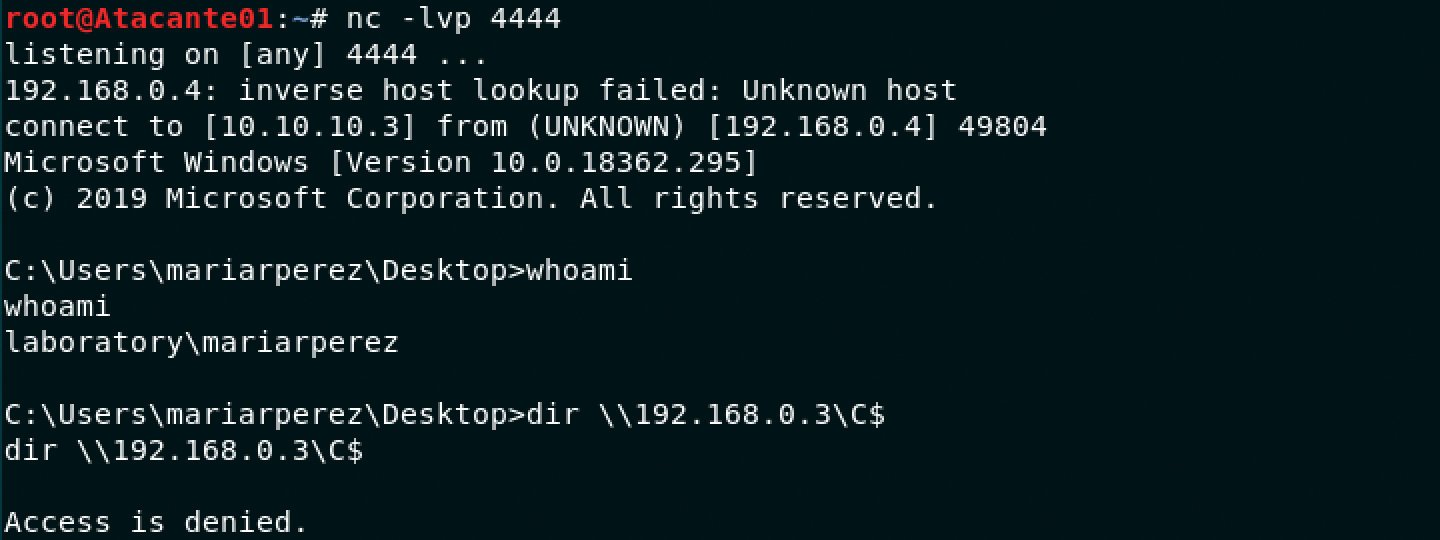
\includegraphics[width=15cm]{PTH/PTH1.png}
\end{center}
\caption{Reverse Shell interactiva sin privilegios.}
\label{PTH1}
\end{figure}

\item Si recogemos el tráfico intercambiado entre la máquina Cliente01 y el DC01, podemos ver que al intentar listar un directorio a través de la IP de éste se realiza a través del protocolo SMB utilizando el protocolo de autenticación NTLM donde el user es {\it LABORATORY\textbackslash{}mariarperez}. Al no tener privilegios, nos deniega el acceso (Figura \ref{PTH2}).
\begin{figure}[H] %[ht!] para here [b] para bottom [t] para top
\begin{center}
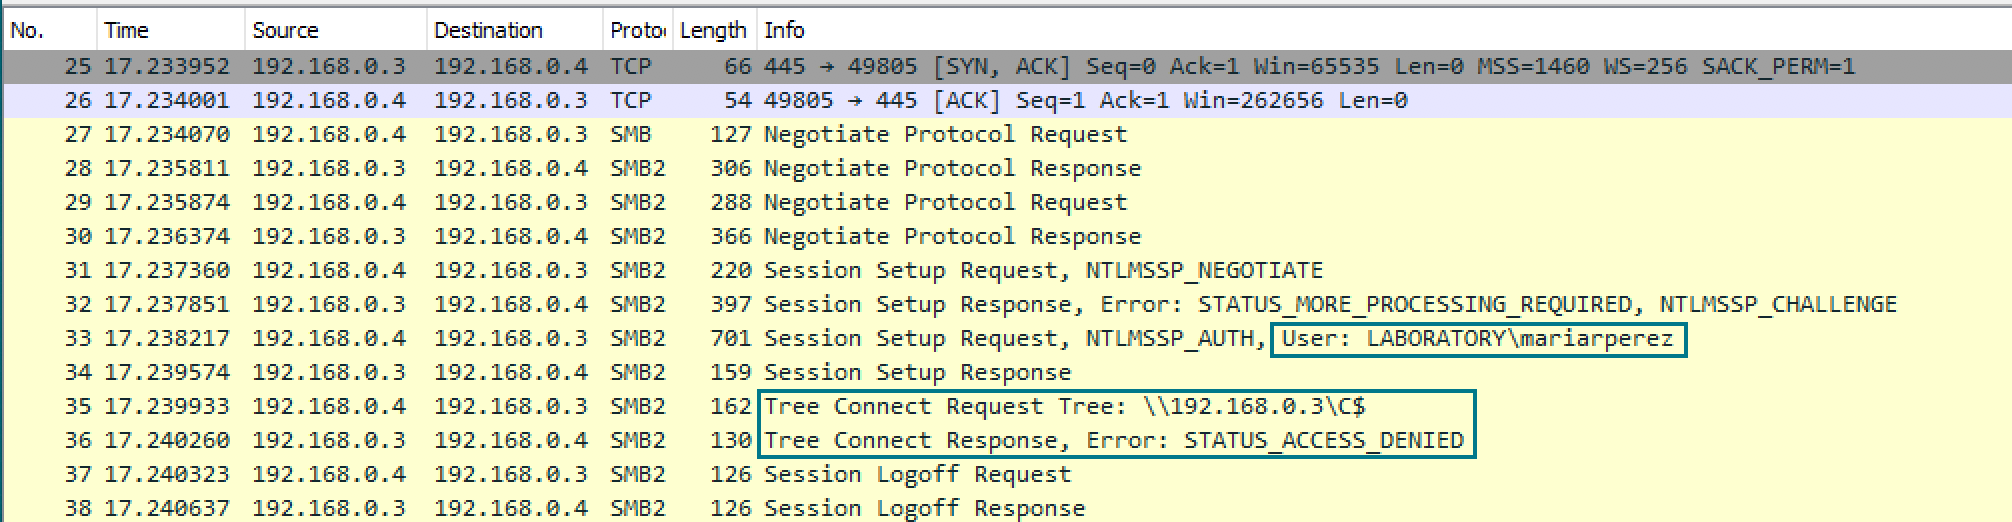
\includegraphics[width=15cm]{PTH/PTH2.png}
\end{center}
\caption{Paquetes intercambiados entre Cliente01 y DC01 - Sin pass the hash.}
\label{PTH2}
\end{figure}

\item  Al disponer de una sesión válida el usuario {\it federicogar} podemos obtener el hash de la contraseña del proceso LSASS. Para ello, se ha utilizado la herramienta Mimikatz~\cite{Capitulo5:Mimikatz} a través de los siguientes comandos (Figura \ref{PTH3}).
\begin{listing}[style=consola, numbers=none]
# privilege::debug
# sekurlsa::logonpasswords
\end{listing}

\begin{figure}[H] %[ht!] para here [b] para bottom [t] para top
\begin{center}
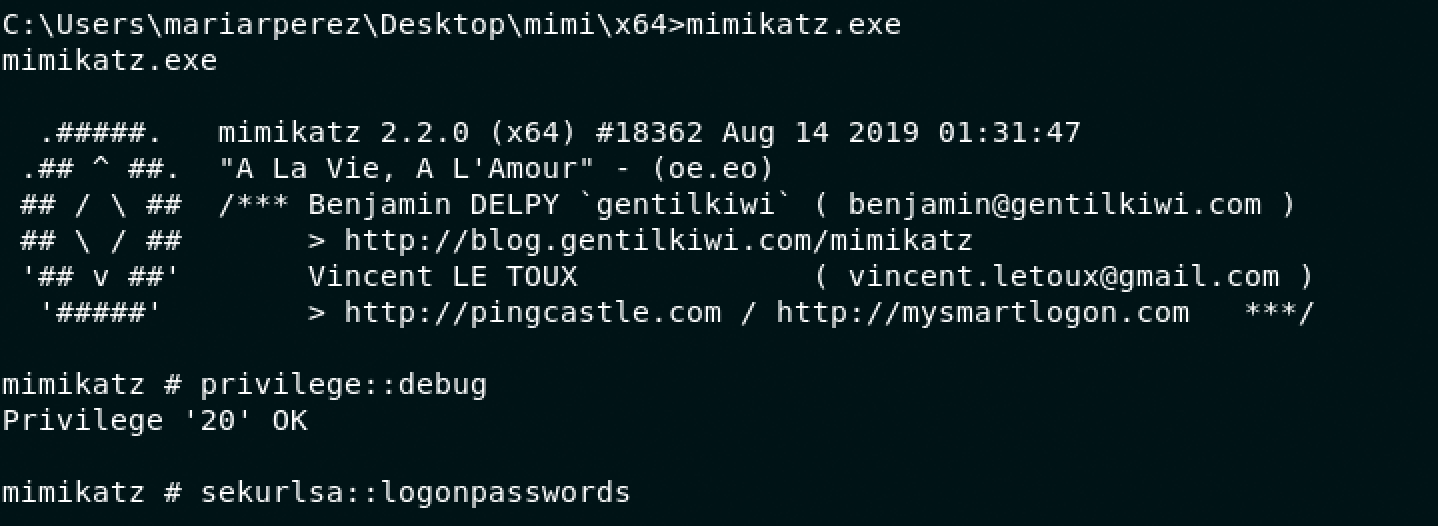
\includegraphics[width=15cm]{PTH/PTH3.png}
\end{center}
\caption{Comandos Mimikatz para listas sesiones activas.}
\label{PTH3}
\end{figure}

\item El comando anterior lista todos las sesiones activas en el usuario, por lo tanto, buscamos la que pertenece al usuario víctima y obtenmos el Hash NT (Figura \ref{PTH4}).
\begin{figure}[H] %[ht!] para here [b] para bottom [t] para top
\begin{center}
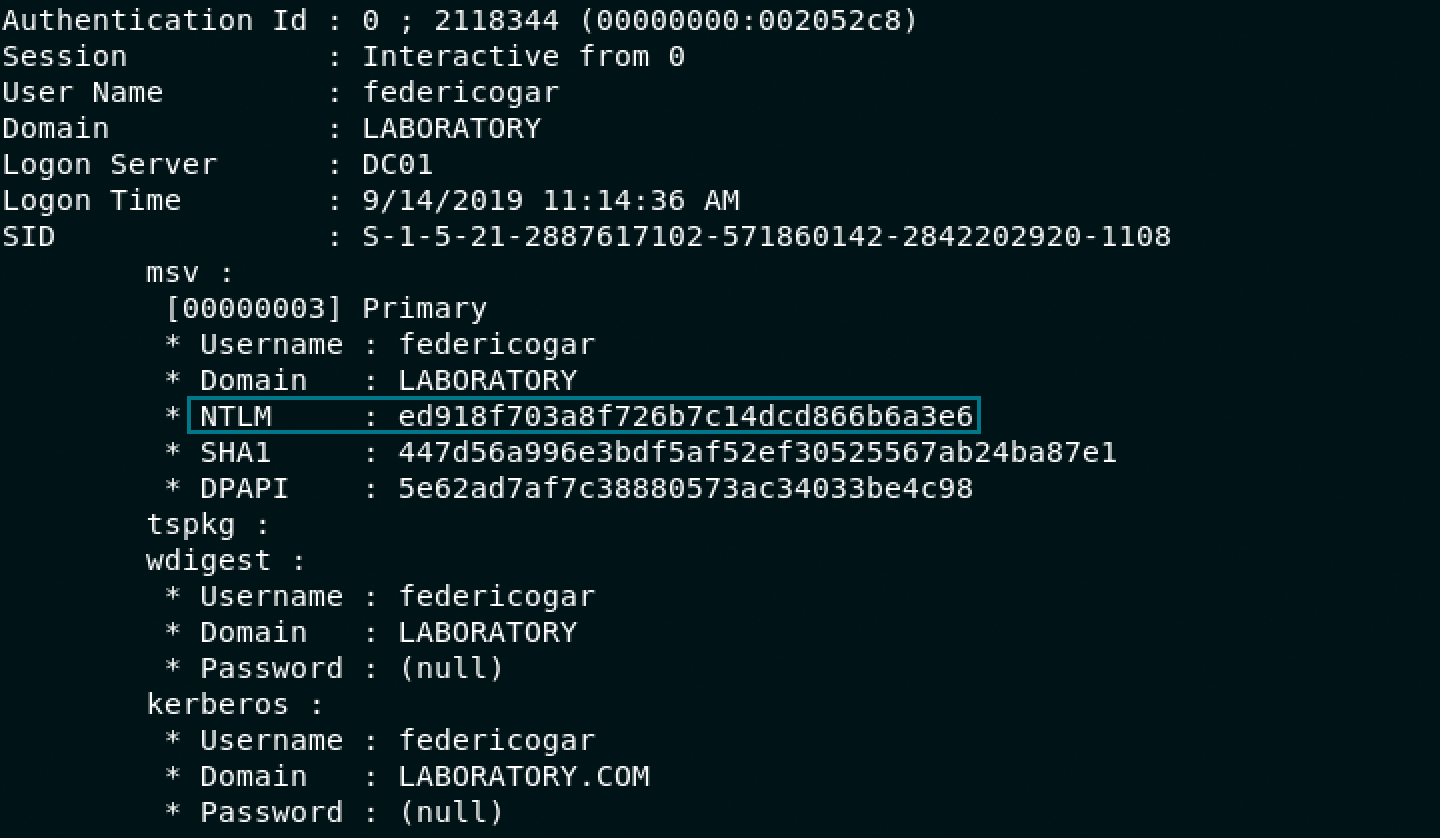
\includegraphics[width=15cm]{PTH/PTH4.png}
\end{center}
\caption{Hash del usuario víctima.}
\label{PTH4}
\end{figure}

\item La propia herramienta Mimikatz permite realizar el ataque Pass the Hash a través del siguiente comando, el resultado de este comando se puede observar en la Figura \ref{PTH5}.
\begin{listing}[style=consola, numbers=none]
# sekurlsa::pth /user:federicogar /ntlm:ed918f703a8f726b7c14dcd866b6a3e6 /domain:LABORATORY /run:cmd.exe
\end{listing}


\begin{figure}[H] %[ht!] para here [b] para bottom [t] para top
\begin{center}
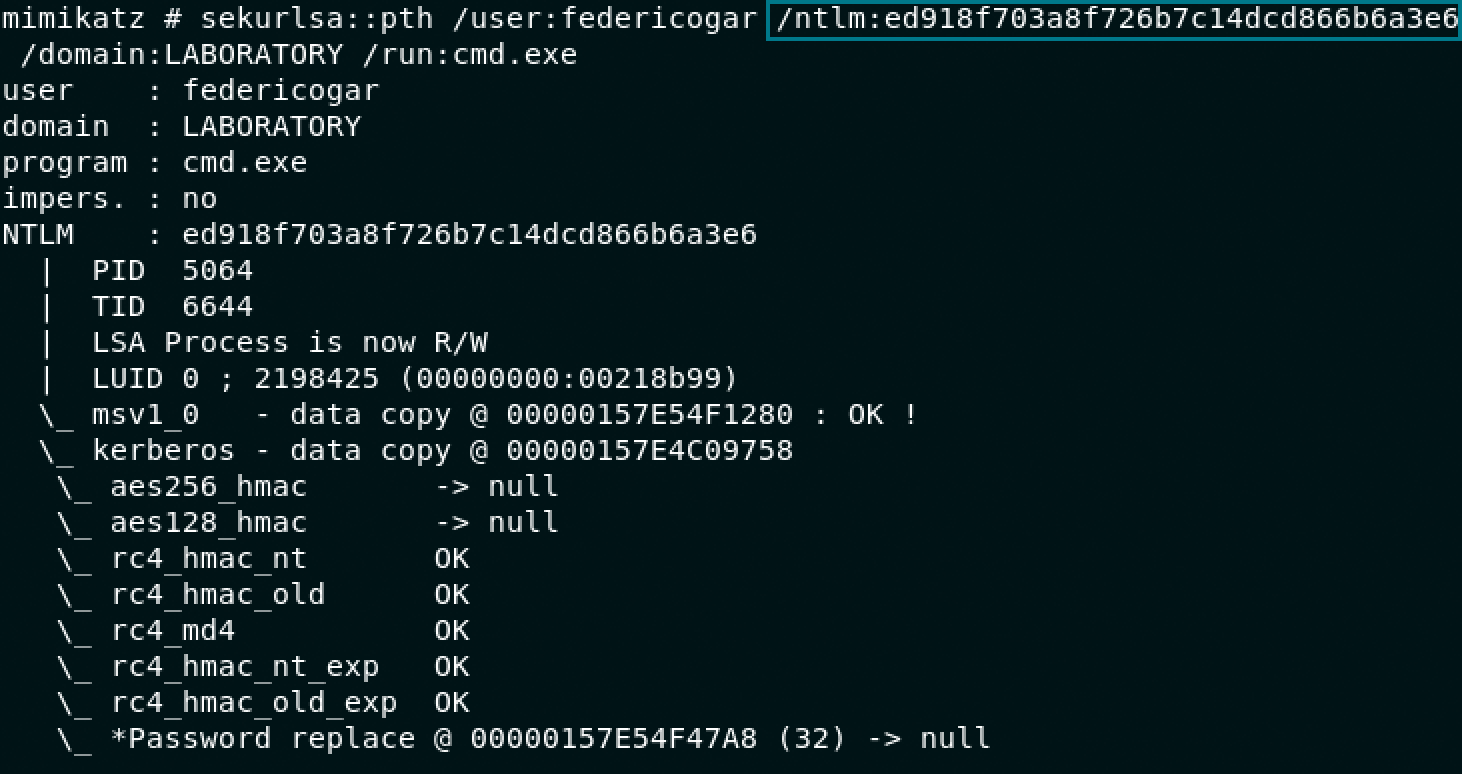
\includegraphics[width=15cm]{PTH/PTH5.png}
\end{center}
\caption{Pash the hash a través de la herramienta Mimikatz.}
\label{PTH5}
\end{figure}

\item En el comando anterior, se definió que ejecutar el comando {\it cmd.exe}, este comando se ejecutará en el Cliente01, por lo tanto, si queremos que se ejecute otra {\it Reverse Shell} con privilegios del uusario víctima sería necesario especificar otro comando. En la shell resultante (Figura \ref{PTH6}) podemos observar que aunque seguimos siendo el uusario {\it mariarperez} podemos listar los archivos de DC01. Esto es debido a que Mimikatz genera una nueva sesión para el usuario {\it mariarperez} y sobreescribe el contenido de las credenciales con el hash del otro usuario. 
\begin{figure}[H] %[ht!] para here [b] para bottom [t] para top
\begin{center}
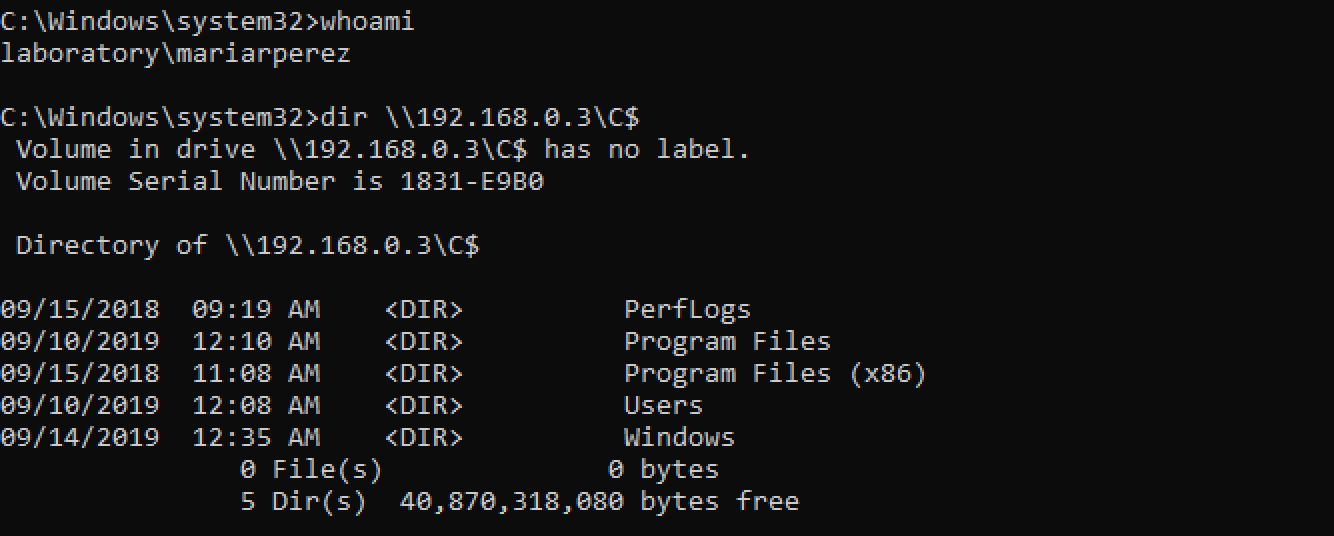
\includegraphics[width=15cm]{PTH/PTH6.png}
\end{center}
\caption{Ataque pass the hash realizado correctamente.}
\label{PTH6}
\end{figure}

\item Por último, al recoger el tráfico generado en esta comunicación podemos observar bastantes diferencias con la figura anterior, ahora el usuario es {\it federicogar} y se ha realizado el {\it Challenge-Response} de NTLM satisfactoriamente pudiendo listar los ficheros (Figura \ref{PTH7}).
\begin{figure}[H] %[ht!] para here [b] para bottom [t] para top
\begin{center}
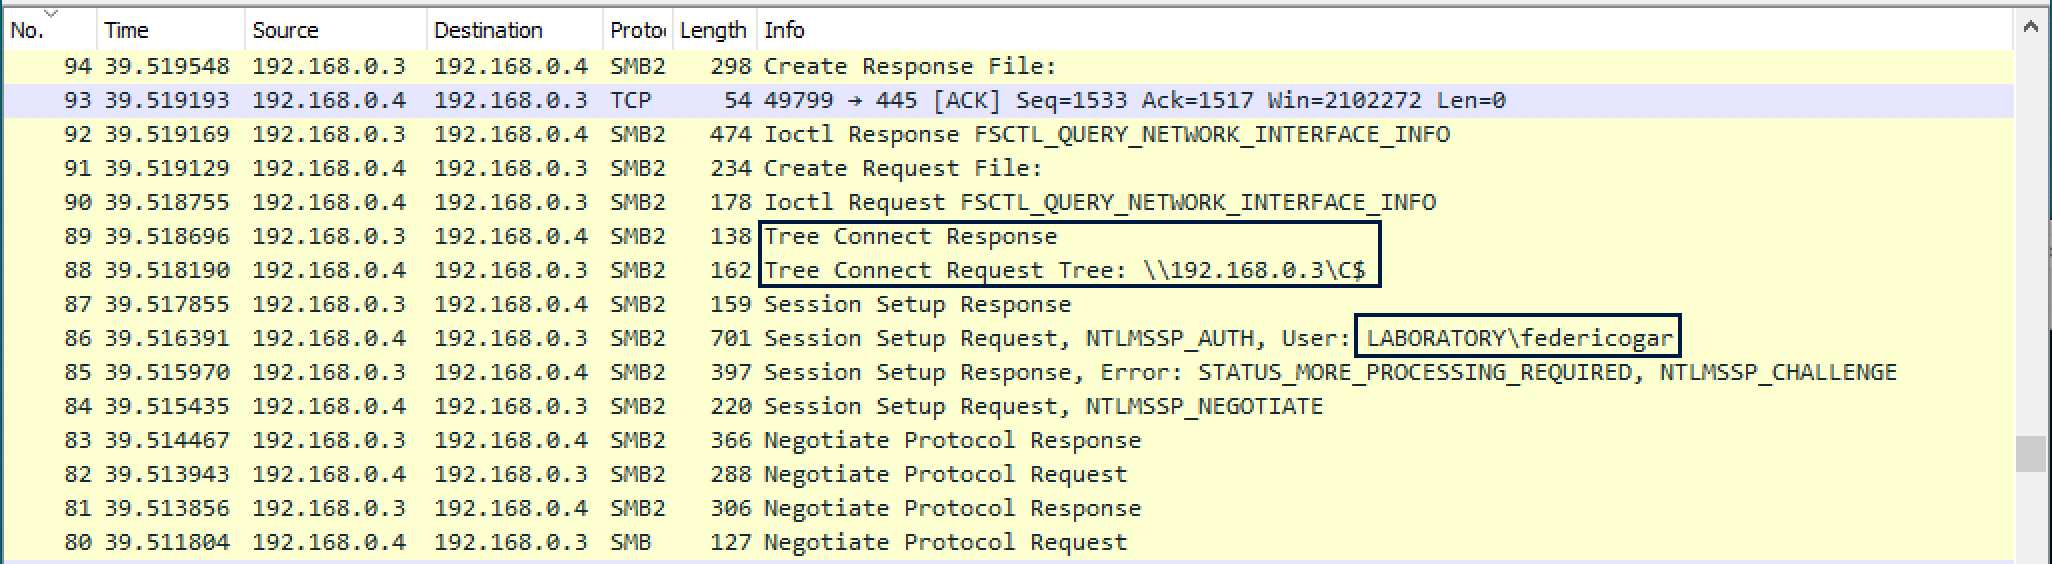
\includegraphics[width=15cm]{PTH/PTH7.png}
\end{center}
\caption{Paquetes intercambiados entre Cliente01 y DC01 - Con pass the hash.}
\label{PTH7}
\end{figure}

\end{enumerate}

\section{NTLM Relay}

Hoy en día los ataques de {\it NTLM Relay} son un técnica muy utilizada por {\it Pentesters} y atacantes permitiendo el acceso a activos o recursos crítico incluso si la organización dispone de buenas prácticas para la gestión de la seguridad. A grandes rasgos, esta técnica de movimiento lateral o vertical se puede sintetizar como un ataque de {\it pass the hash} pero a nivel de red. \\ 

Para entender este ataque es necesario entender el protocolo {\it Challenge - Respuesta} utilizado por NTLM. Aunque se ha detallado anteriormente se puede sintetizar en las siguientes fases: 

\begin{enumerate}
\item El cliente intenta iniciar sesión en un servicio o recurso.
\item El servidor responde con un desafío o {\it challenge}, es decir, el cliente dice, si eres quién dice ser, cifra este desafío con tu hash de la contraseña..
\item El cliente cifra el desafío.
\item El servidor compueba este cifrado descifradno el desafió ya que dispone del hash del usuario, si es correcto verifica al usuario. 
\end{enumerate}

En un ataque de NTLM Relay, el atacante se sitúa como intermediario entre los paquetes intercambiados en el proceso anterior. Para ello, selecciona el recurso o activo que quiere autenticarse y espera a que un usuario legítimo intente conectarse a él. A continuación se va a detallar cómo cambia el esquema de autenticación NTLM cuando se está produciendo un ataque de {\it NTLM Relay}~\cite{Capitulo5:NTLMRelay}:

\begin{enumerate}
\item En primer lugar, el cliente intenta conectarse a un recuso, esta petición es interceptada por un atacante y reenviada al servidor objetivo. 
\item El servidor contesta con un desafío, este desafío también es interceptado por el atacante y reenviado a la víctima.
\item La víctima cifra con el Hash NT de la contraseña el desafío y crea un paquete que será enviado de nuevo al atacante y este lo reenviará al servidor. 
\item El servidor comprueba que el desafío se ha cifrado correctamente y concede el acceso a dicho recurso. Por lo tanto, el atacante tiene acceso a ese recurso ya que dispone del paquete con el desafío cifrado. 
\item Por último, el atacante manda un paquete a la vítima denegando el acceso a ese recurso. 
\end{enumerate}

Como es de esperar, este tipo de ataques ha sido perseguido de cerca por Microsoft y ha implementado medidas que dificultan o imposibilitan este ataque. Una de ellas es el parche MS08-068~\cite{Capitulo5:MS08-068} que imposibilita que se puede retrasmitir un Hash NTLM a la misma máquina de la que se obtuvo imposibilitando así los ataques de NTLM Replay reflejado. Sin embargo, estos hashes se pueden retrasmitir a otros servicios o máquinas. \\

Para replicar este tipo de ataque sen el laboratorio local se va a utilizar la herramienta Responder~\cite{Capitulo5:Responder}. Antes de definir esta herramienta es necesario hablar de los {\it Windows Name Resolution}, es decir, de la forma que utilizada Microsoft para resolver los nombres de dominio. Para ello, se utilizan los protocolos: {\it Link Local Multicast Name Resolution (LLMNR)} y {\it NetBIOS over TCP/IP Name Service}. La herramienta Responder realiza un ``envenamiento'' de estos protocolos y permite obtener la credenciales en red. Esta herramienta crea servidores de autenticación como puede ser SMB, MYSQL, HTTP(s), FTP... y obliga a la víctima a enviar las credenciales a estos servidores y así poder obtenerlas. \\

Por lo tanto, con la herramienta Responder podemos obtener los Hashes NTLM de una conexión de autenticación y retrasmitirlos a través de otra herramienta como puede ser {\it ntlmrelayx.py} de la librería de Impacket o {\it MultiRelay.py}. \\

Una de las limitaciones de este ataque es que la medida que implementó Windows: SMB Signing~\cite{Capitulo5:SMBSigning} debe estar desactivado. Esta medida firma los paquetes SMB para evitar que estos sean modificados durante su retrasmisión. Se puede suponer que esta medida esta desactivada ya que en la mayoría de los Sistemas Windows están desactivadas a escepción de Windows Server como se puede ver en la Figura \ref{NTLMRelay1}.

\begin{figure}[H] %[ht!] para here [b] para bottom [t] para top
\begin{center}
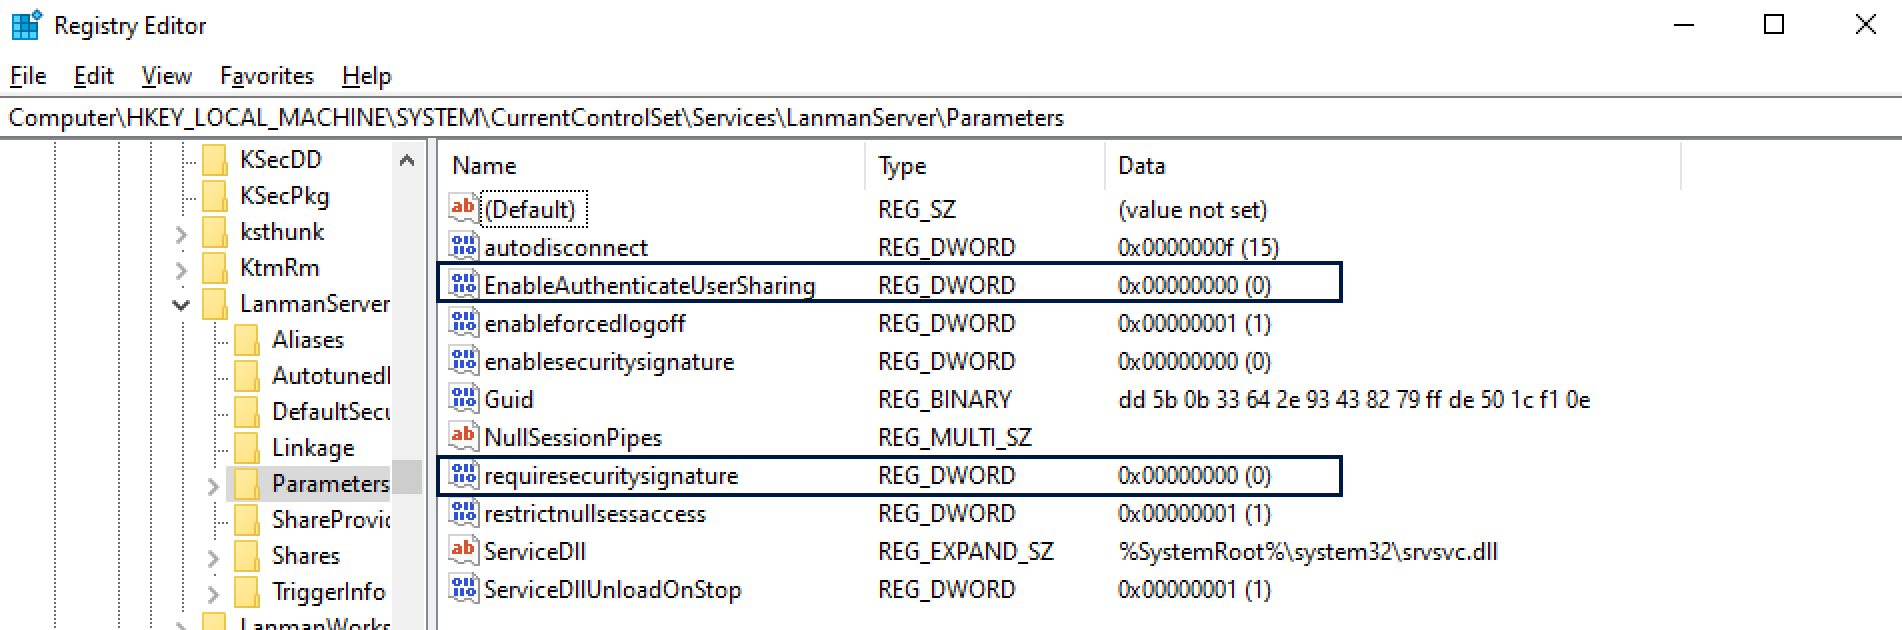
\includegraphics[width=15cm]{NTLMRelay/NTLMRelay1.png}
\end{center}
\caption{SMB Signing desactivado por defecto en Cliente01.}
\label{NTLMRelay1}
\end{figure}

\subsubsection{Experimentación}

Para ejecutar este ataque, la máquina Atacante01 tiene que estar en la misma red, para ello, desde VirtualBox añadimos una nueva tarjeta de red que esté conectada a ADNET y le asignamos la dirección IP: 192.168.0.5.

\begin{enumerate}

\item En primer lugar, descargamos la última versión de Responder de ~\cite{Capitulo5:Responder} o se utiliza la versión que trae por defecto Kali Linux, en cualquier caso se debe editar el archivo {\it Responder.conf} y deshabilitar las opciones SMB y HTTP para que estas peticiones sean recogidas por {\it ntlmrelayx.py} (Figura \ref{NTLMRelay2}
\begin{figure}[H] %[ht!] para here [b] para bottom [t] para top
\begin{center}
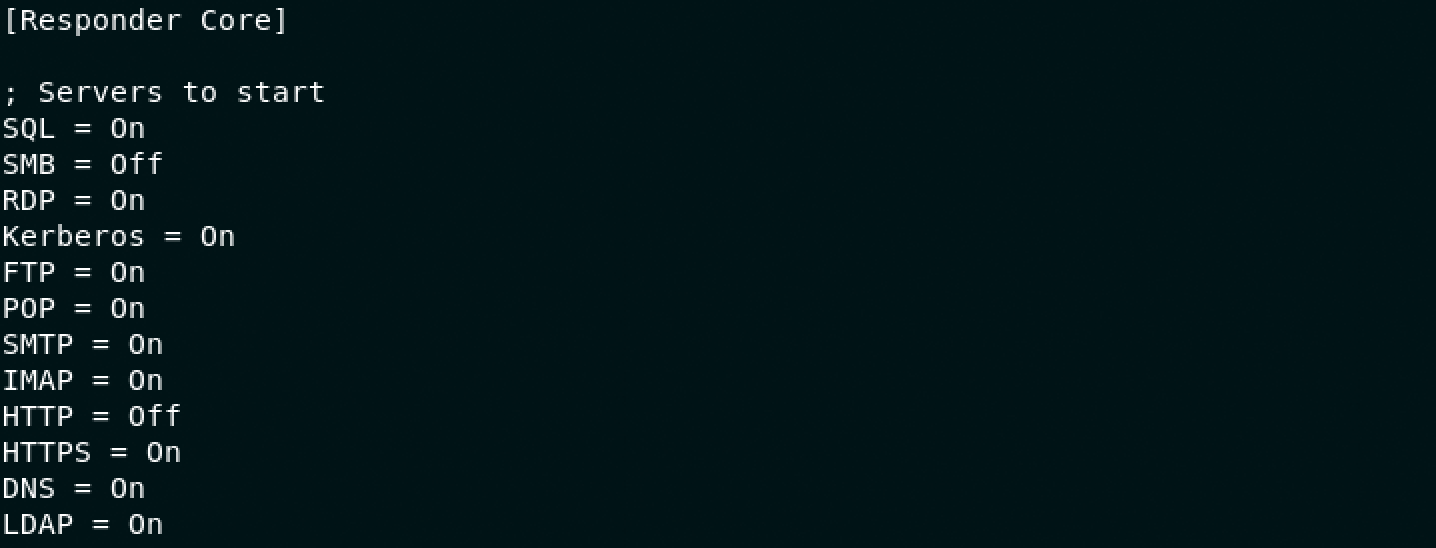
\includegraphics[width=15cm]{NTLMRelay/NTLMRelay2.png}
\end{center}
\caption{Archivo de configuración Responder.conf.}
\label{NTLMRelay2}
\end{figure}

\item Una vez editada la configuración ejecutamos el Responder. En paralelo en otra terminal ejecutamos el {\it ntlmrelayx.py} (Figura \ref{NTLMRelay3}) a través de los siguientes comandos:

\begin{listing}[style=consola, numbers=none]
# .\Responder.py -I eth2 -w -r -f -v
# ntlmrelayx.py -t 192.168.0.3 -smb2support
\end{listing}

-I eth2 - Corresponde con la interfaz de red conectada a la ADNET.
-t 192.168.0.3 - Corresponde al target, en este caso DC01. 

\begin{figure}[H] %[ht!] para here [b] para bottom [t] para top
\begin{center}
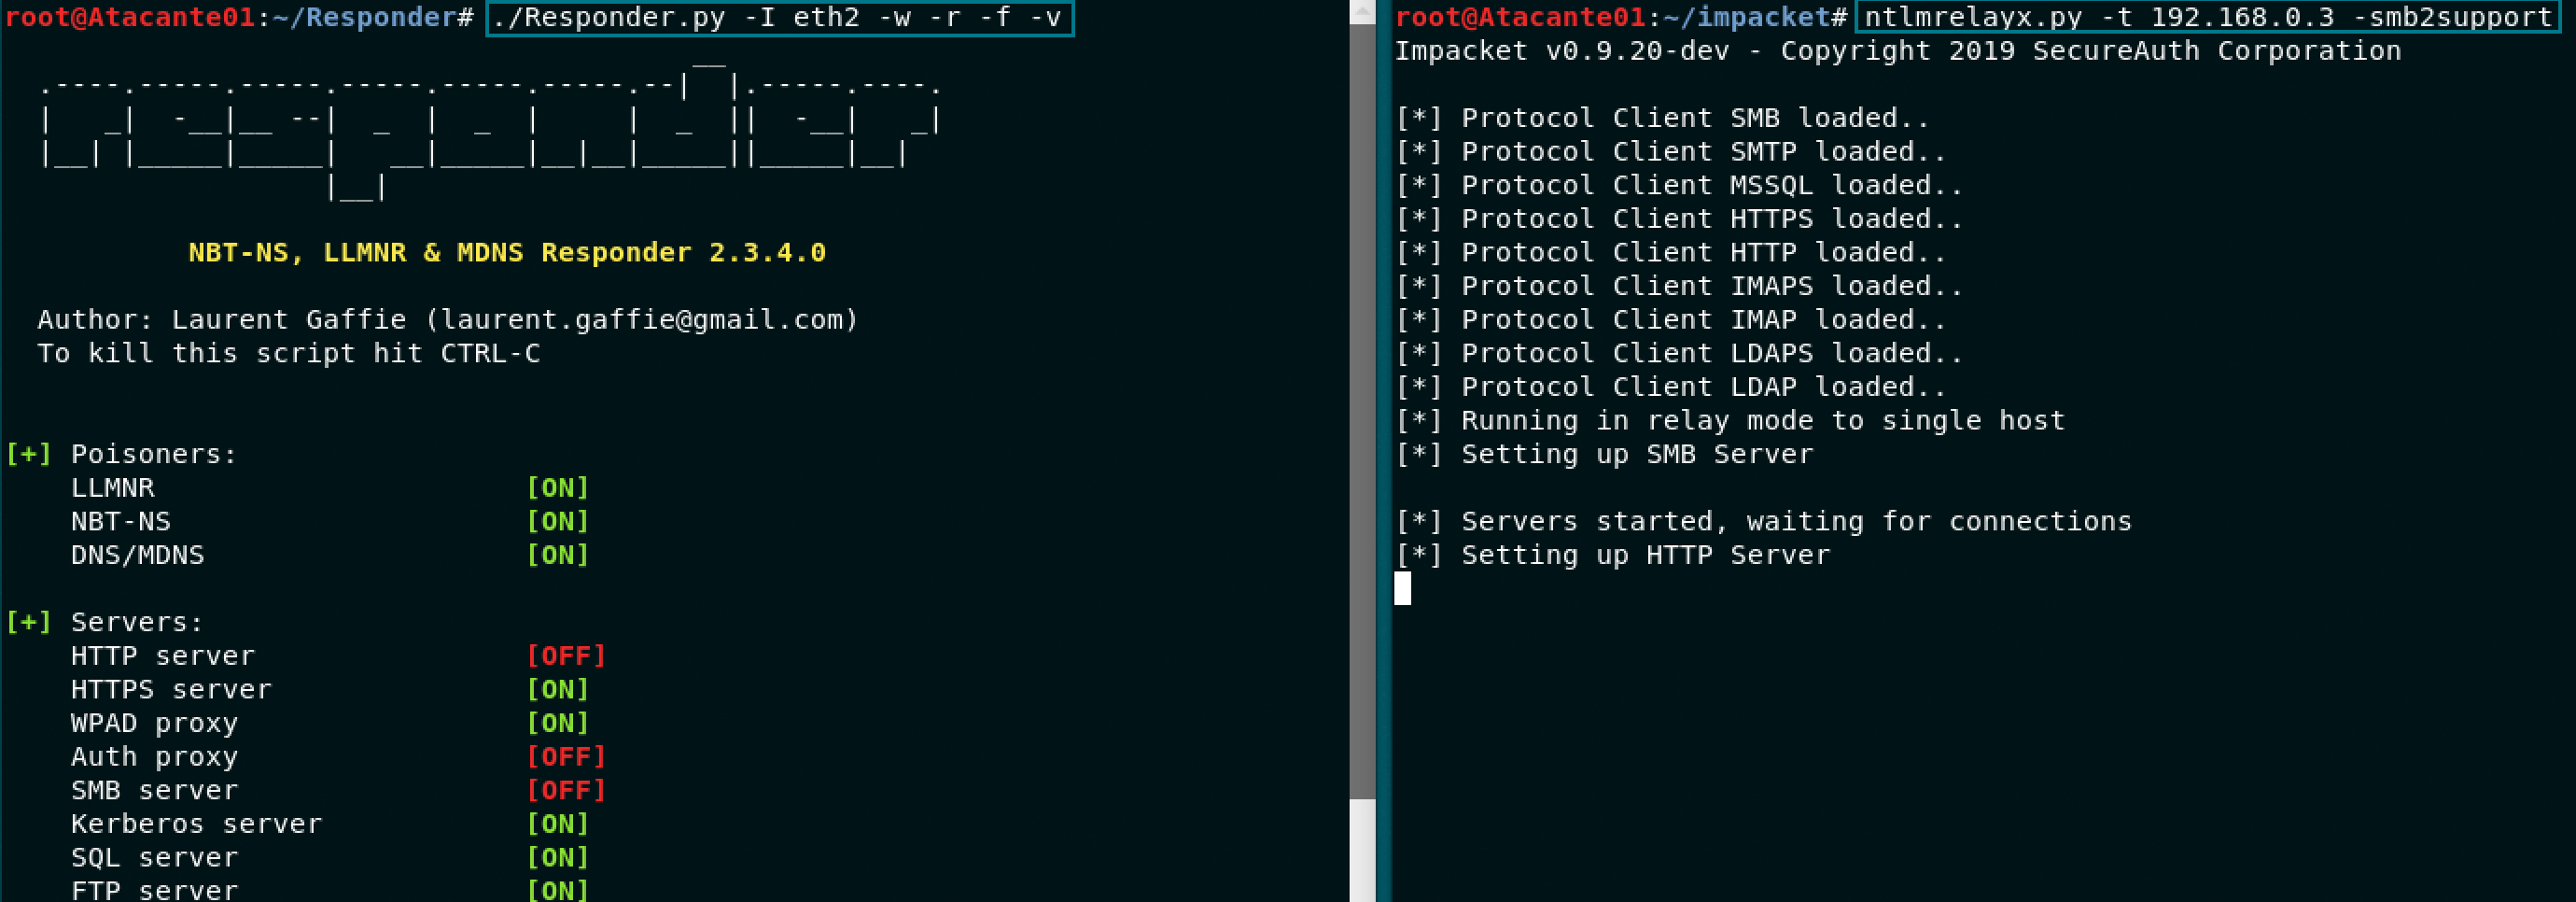
\includegraphics[width=15cm]{NTLMRelay/NTLMRelay3.png}
\end{center}
\caption{Responder y ntlmrelayx.py.}
\label{NTLMRelay3}
\end{figure}

\item Para que este ataque funcione se necesita la interacción del usuario víctima, en este caso bastaría que el usuario con privilegios de Domain Admin se conectara a un recurso inexistente como puede ser \footnote{\textbackslash{}\textbackslash{}test\textbackslash{}C\$} (Figura \ref{NTLMRelay4}).
\begin{figure}[H] %[ht!] para here [b] para bottom [t] para top
\begin{center}
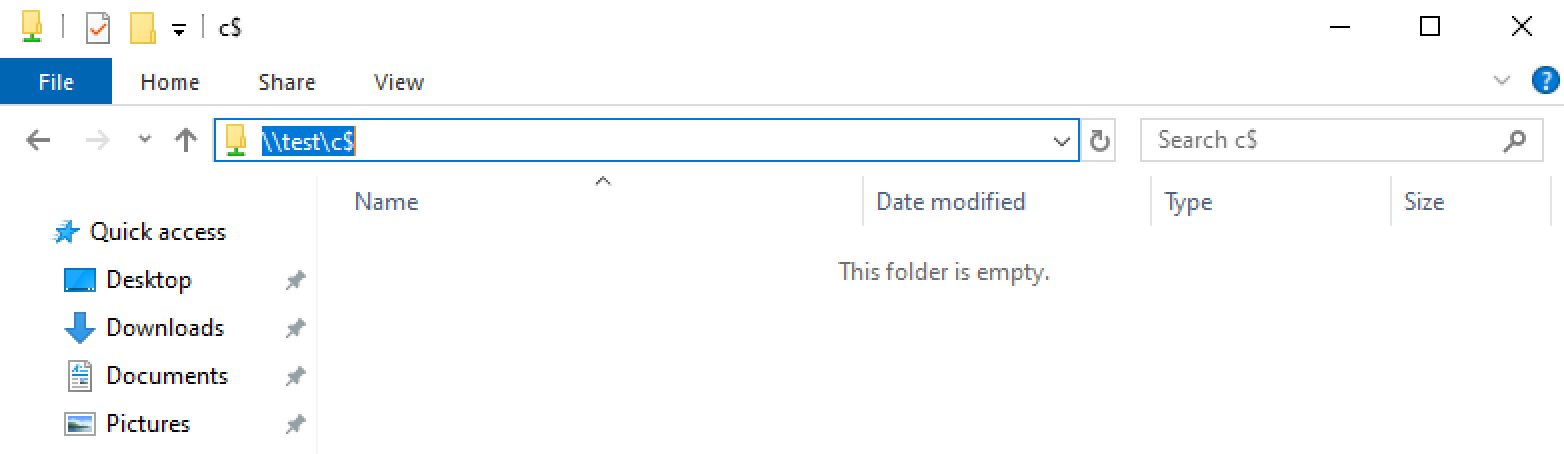
\includegraphics[width=15cm]{NTLMRelay/NTLMRelay4.png}
\end{center}
\caption{Interacción del usuario.}
\label{NTLMRelay4}
\end{figure}

\item Como se puede ver en la Figura \ref{NTLMRelay5} el ataque se ejecuta correctamente y se vuelca los datos de la SAM del Domain Controller. 
\begin{figure}[H] %[ht!] para here [b] para bottom [t] para top
\begin{center}
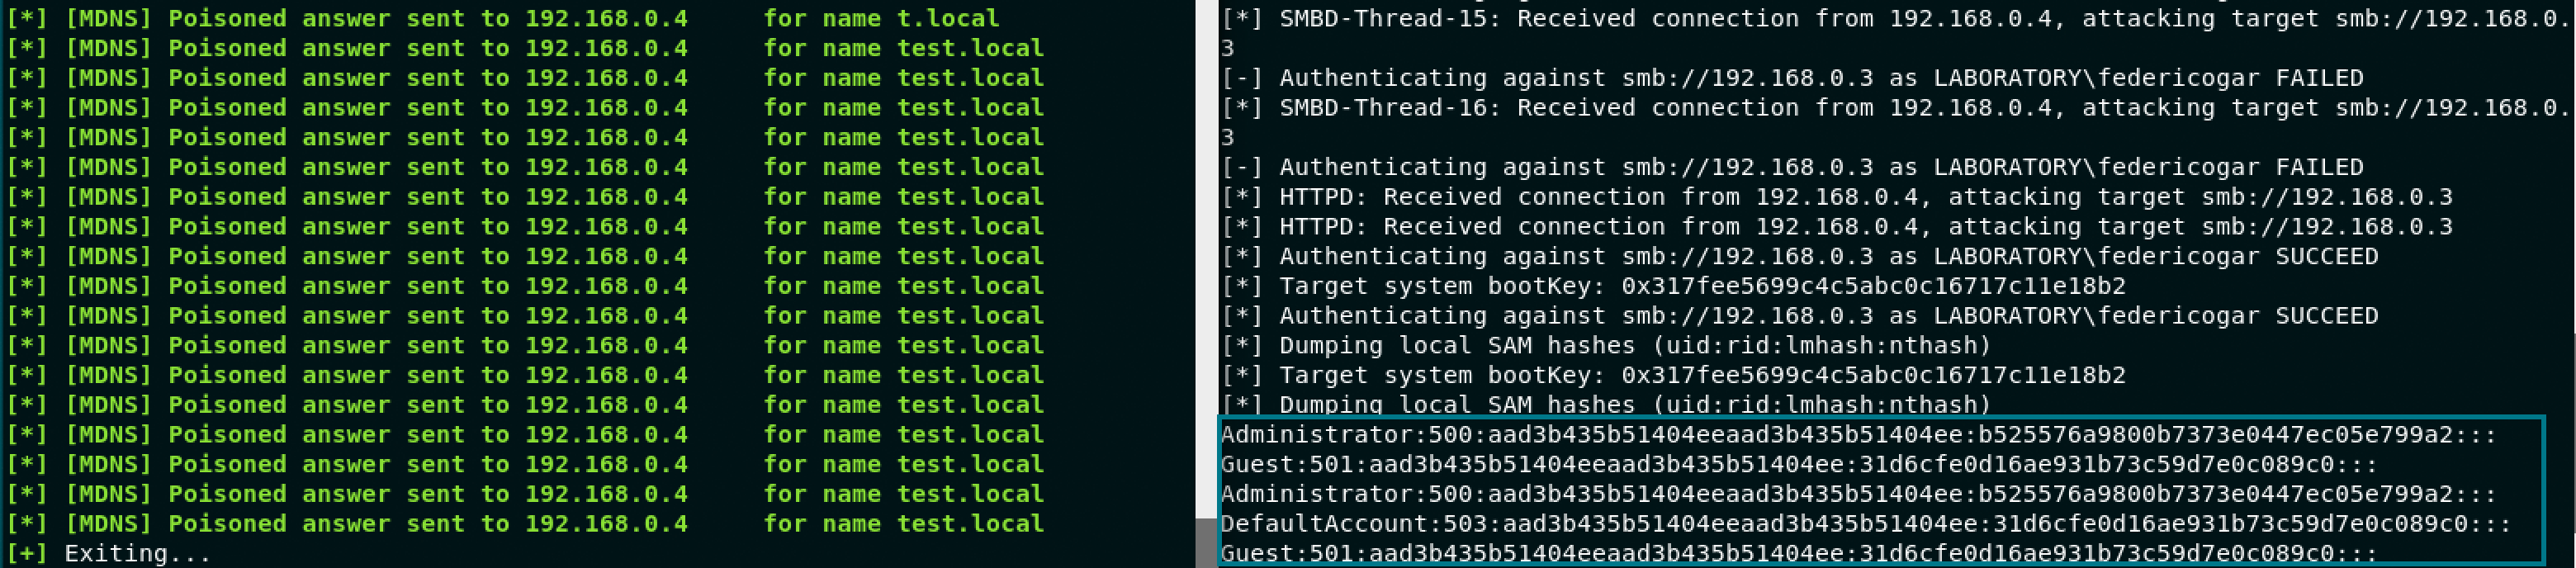
\includegraphics[width=15cm]{NTLMRelay/NTLMRelay5.png}
\end{center}
\caption{Volcado de la SAM.}
\label{NTLMRelay5}
\end{figure}

\end{enumerate}

\section{Overpass The Hash}

La técnica {\it Overpass the hash}, también conocida como {\it Pass the key (PTK)} es la equivalencia a {\it Pass the hash} para el protocolo de autenticación Kerberos. Como se ha visto anteriormente, durante el intercambio de paquetes, el usuario cifra una marca de tiempo o {\it timestamp}. En función de la versión de Kerberos se va a utilizar un secreto u otro, en este caso en las versiones más antiguas utiliza un secreto RC4 que equivale al Hash NT del usuario, en versiones más modernas utiliza claves de AES128 y AES256. Por lo tanto, con el Hash NT del usuario se puede obtener un Ticket TGT y poder realizar la autenticación correctamente.

\subsubsection{Experimentación}

\begin{enumerate}
\item En primer lugar, partimos desde una {\it Reverse Shell} interactiva con privilegios de administrador del usuario {\it mariarperez} y tratamos de listar el directorio {\it C\$} del DC01 a través de protocolo de Kerberos(Figura \ref{OTH1}).
\begin{figure}[H] %[ht!] para here [b] para bottom [t] para top
\begin{center}
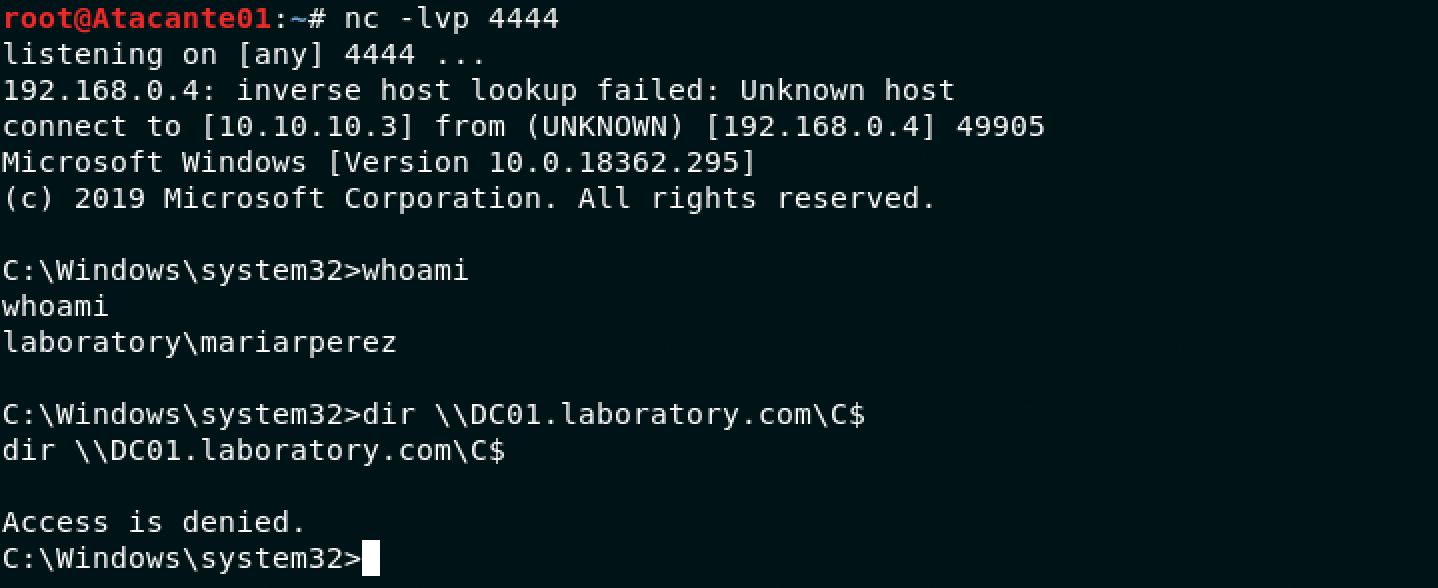
\includegraphics[width=15cm]{OTH/OTH1.png}
\end{center}
\caption{Reverse Shell interactiva.}
\label{OTH1}
\end{figure}

\item Como se puede ver en Wireshark, el intercambio de paquetes KRB5 falla (Figura \ref{OTH2}).
\begin{figure}[H] %[ht!] para here [b] para bottom [t] para top
\begin{center}
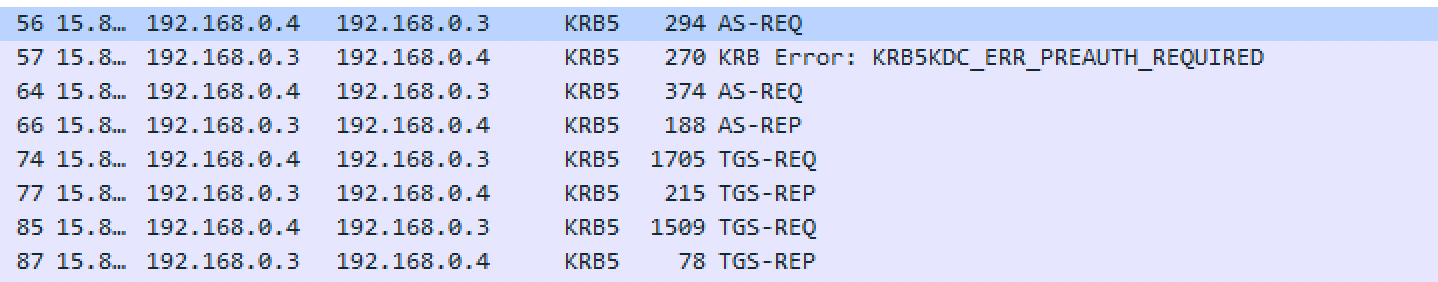
\includegraphics[width=15cm]{OTH/OTH2.png}
\end{center}
\caption{Intercambio de paquetes de Kerberos.}
\label{OTH2}
\end{figure}

\item Repetimos los pasos hechos en {\it Pass the hash}, listamos las sesiones activas y obtenemos el hash de la contraseña MD5 (Figura \ref{OTH3} y Figura \ref{OTH4}).
\begin{figure}[H] %[ht!] para here [b] para bottom [t] para top
\begin{center}
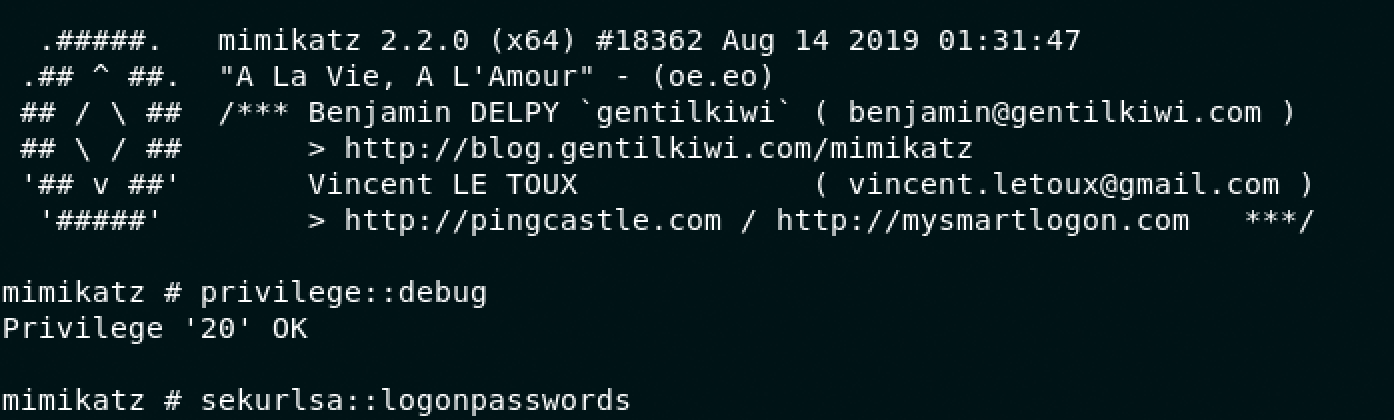
\includegraphics[width=15cm]{OTH/OTH3.png}
\end{center}
\caption{Comandos Mimikatz para listas sesiones activas.}
\label{OTH3}
\end{figure}

\begin{figure}[H] %[ht!] para here [b] para bottom [t] para top
\begin{center}
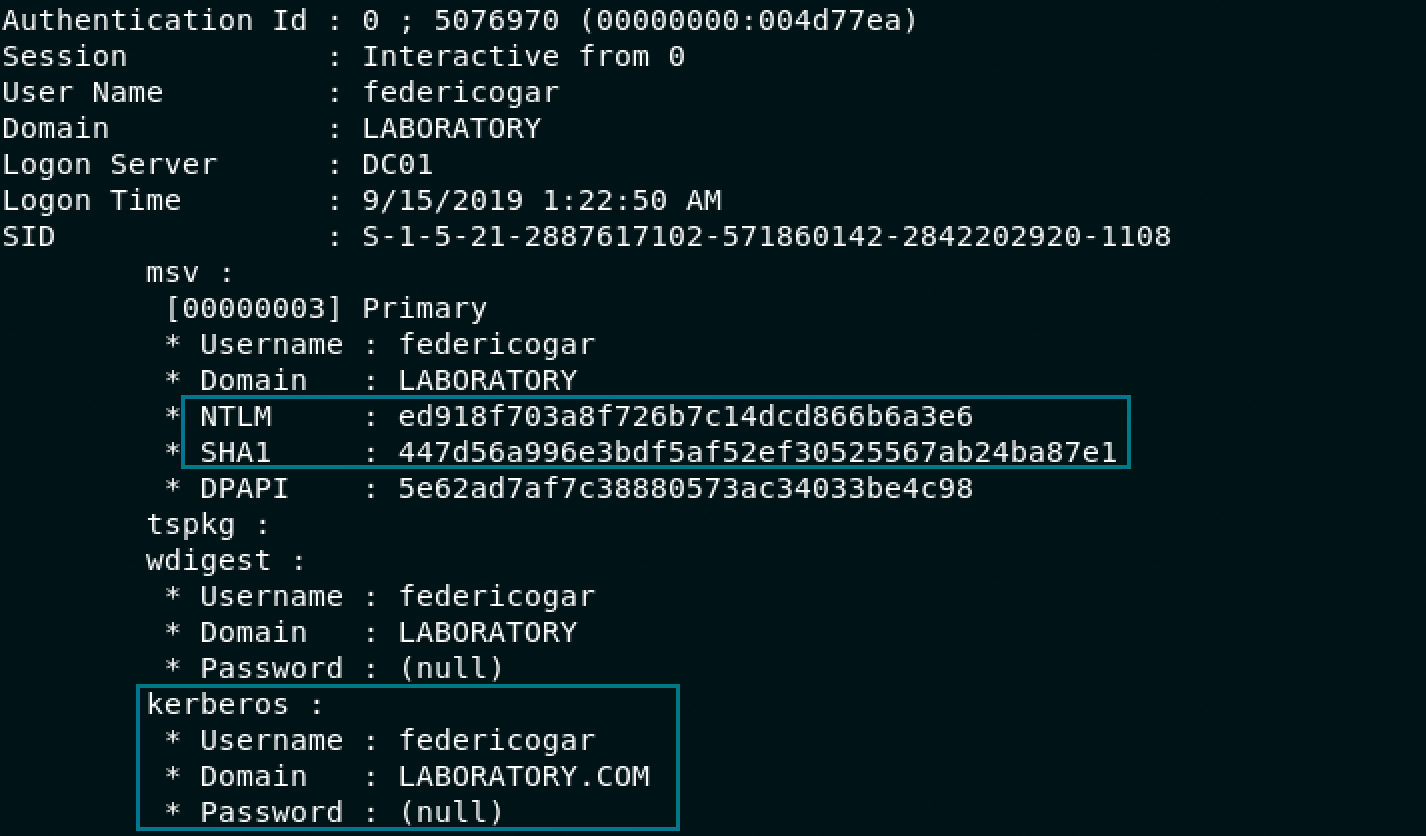
\includegraphics[width=15cm]{OTH/OTH4.png}
\end{center}
\caption{Hash del usuario víctima.}
\label{OTH4}
\end{figure}

\item Realizamos el ataque a través del mismo comando que en {\it Pass the hash} (Figura \ref{OTH5}).
\begin{figure}[H] %[ht!] para here [b] para bottom [t] para top
\begin{center}
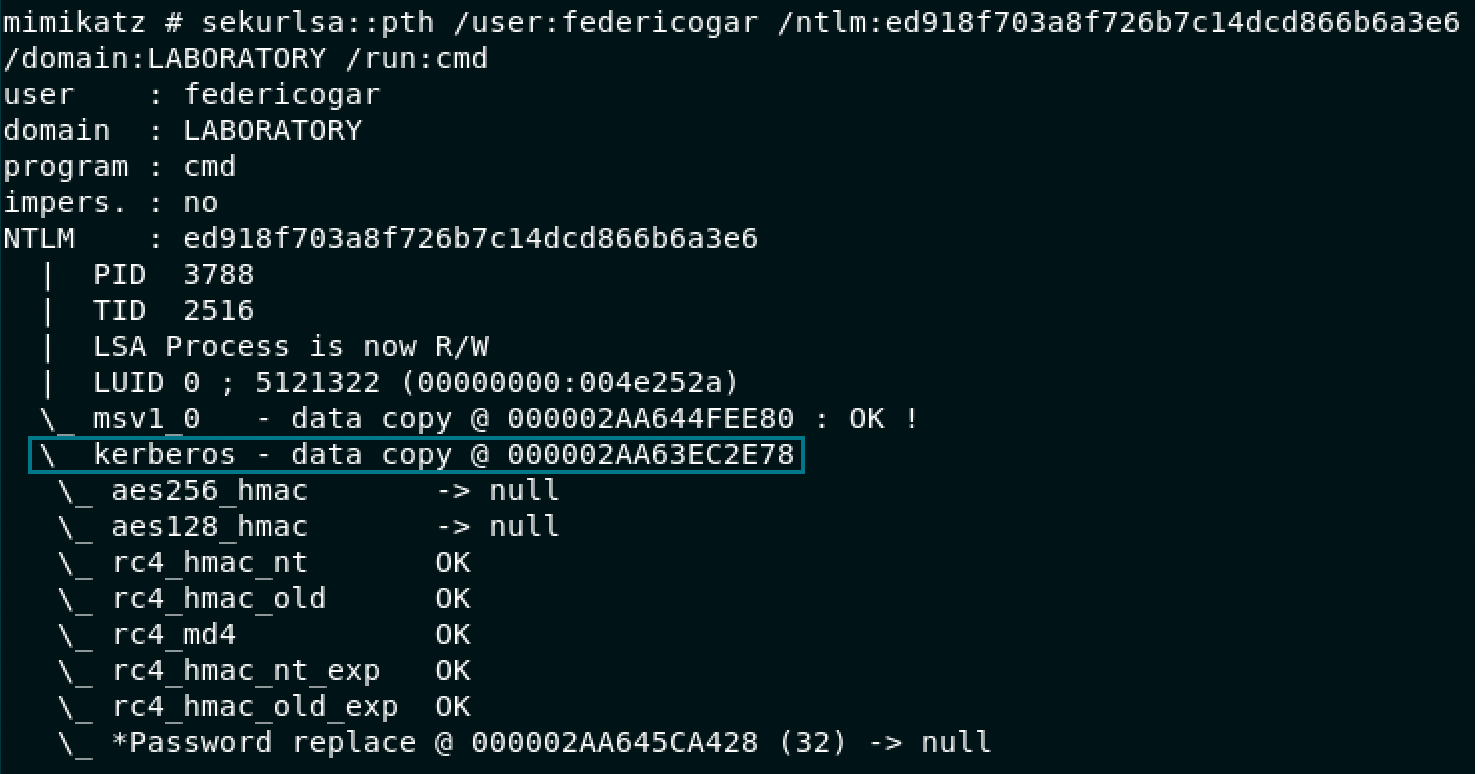
\includegraphics[width=15cm]{OTH/OTH5.png}
\end{center}
\caption{Pash the hash a través de la herramienta Mimikatz.}
\label{OTH5}
\end{figure}

\item Se ejecuta el comando especificado en el comando anterior, en este caso un {\it cmd.exe} en el que podemos acceder al directorio (Figura \ref{OTH6}).
\begin{figure}[H] %[ht!] para here [b] para bottom [t] para top
\begin{center}
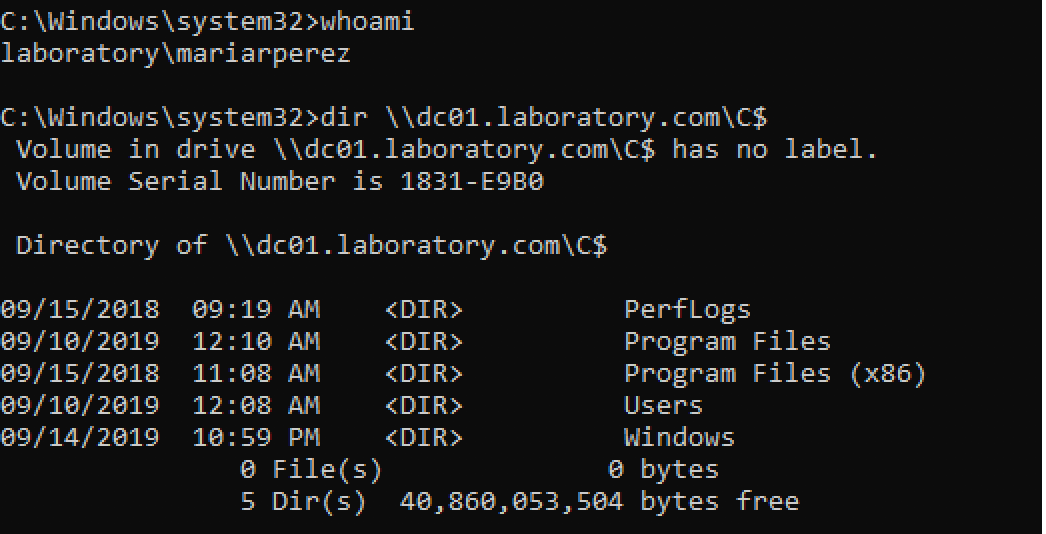
\includegraphics[width=15cm]{OTH/OTH6.png}
\end{center}
\caption{Ataque over-pass the hash realizado correctamente..}
\label{OTH6}
\end{figure}

\item En los paquetes KRB5 intercambiados podemos ver que se usa RC4 (Figura \ref{OTH7}) y que la autenticación se completa correctamente recibiendo así un Ticket TGT. 
\begin{figure}[H] %[ht!] para here [b] para bottom [t] para top
\begin{center}
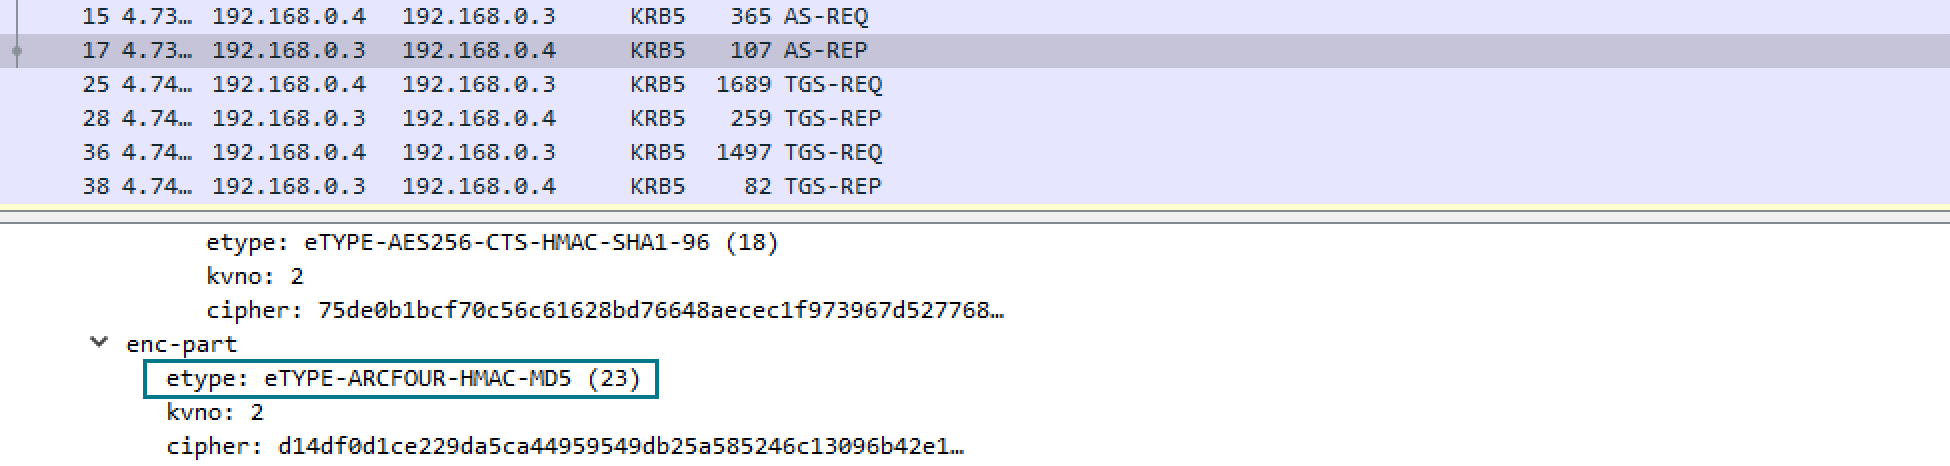
\includegraphics[width=15cm]{OTH/OTH7.png}
\end{center}
\caption{Intercambio de paquetes de Kerberos.}
\label{OTH7}
\end{figure}


\end{enumerate}




\section{Pass The Ticket}

\section{Golden/Silver Ticket}

asection{Kerberoast}
